\documentclass[twoside]{book}

% Packages required by doxygen
\usepackage{fixltx2e}
\usepackage{calc}
\usepackage{doxygen}
\usepackage[export]{adjustbox} % also loads graphicx
\usepackage{graphicx}
\usepackage[utf8]{inputenc}
\usepackage{makeidx}
\usepackage{multicol}
\usepackage{multirow}
\PassOptionsToPackage{warn}{textcomp}
\usepackage{textcomp}
\usepackage[nointegrals]{wasysym}
\usepackage[table]{xcolor}

% Font selection
\usepackage[T1]{fontenc}
\usepackage[scaled=.90]{helvet}
\usepackage{courier}
\usepackage{amssymb}
\usepackage{sectsty}
\renewcommand{\familydefault}{\sfdefault}
\allsectionsfont{%
  \fontseries{bc}\selectfont%
  \color{darkgray}%
}
\renewcommand{\DoxyLabelFont}{%
  \fontseries{bc}\selectfont%
  \color{darkgray}%
}
\newcommand{\+}{\discretionary{\mbox{\scriptsize$\hookleftarrow$}}{}{}}

% Page & text layout
\usepackage{geometry}
\geometry{%
  a4paper,%
  top=2.5cm,%
  bottom=2.5cm,%
  left=2.5cm,%
  right=2.5cm%
}
\tolerance=750
\hfuzz=15pt
\hbadness=750
\setlength{\emergencystretch}{15pt}
\setlength{\parindent}{0cm}
\setlength{\parskip}{3ex plus 2ex minus 2ex}
\makeatletter
\renewcommand{\paragraph}{%
  \@startsection{paragraph}{4}{0ex}{-1.0ex}{1.0ex}{%
    \normalfont\normalsize\bfseries\SS@parafont%
  }%
}
\renewcommand{\subparagraph}{%
  \@startsection{subparagraph}{5}{0ex}{-1.0ex}{1.0ex}{%
    \normalfont\normalsize\bfseries\SS@subparafont%
  }%
}
\makeatother

% Headers & footers
\usepackage{fancyhdr}
\pagestyle{fancyplain}
\fancyhead[LE]{\fancyplain{}{\bfseries\thepage}}
\fancyhead[CE]{\fancyplain{}{}}
\fancyhead[RE]{\fancyplain{}{\bfseries\leftmark}}
\fancyhead[LO]{\fancyplain{}{\bfseries\rightmark}}
\fancyhead[CO]{\fancyplain{}{}}
\fancyhead[RO]{\fancyplain{}{\bfseries\thepage}}
\fancyfoot[LE]{\fancyplain{}{}}
\fancyfoot[CE]{\fancyplain{}{}}
\fancyfoot[RE]{\fancyplain{}{\bfseries\scriptsize Generated by Doxygen }}
\fancyfoot[LO]{\fancyplain{}{\bfseries\scriptsize Generated by Doxygen }}
\fancyfoot[CO]{\fancyplain{}{}}
\fancyfoot[RO]{\fancyplain{}{}}
\renewcommand{\footrulewidth}{0.4pt}
\renewcommand{\chaptermark}[1]{%
  \markboth{#1}{}%
}
\renewcommand{\sectionmark}[1]{%
  \markright{\thesection\ #1}%
}

% Indices & bibliography
\usepackage{natbib}
\usepackage[titles]{tocloft}
\setcounter{tocdepth}{3}
\setcounter{secnumdepth}{5}
\makeindex

% Hyperlinks (required, but should be loaded last)
\usepackage{ifpdf}
\ifpdf
  \usepackage[pdftex,pagebackref=true]{hyperref}
\else
  \usepackage[ps2pdf,pagebackref=true]{hyperref}
\fi
\hypersetup{%
  colorlinks=true,%
  linkcolor=blue,%
  citecolor=blue,%
  unicode%
}

% Custom commands
\newcommand{\clearemptydoublepage}{%
  \newpage{\pagestyle{empty}\cleardoublepage}%
}

\usepackage{caption}
\captionsetup{labelsep=space,justification=centering,font={bf},singlelinecheck=off,skip=4pt,position=top}

%===== C O N T E N T S =====

\begin{document}

% Titlepage & ToC
\hypersetup{pageanchor=false,
             bookmarksnumbered=true,
             pdfencoding=unicode
            }
\pagenumbering{roman}
\begin{titlepage}
\vspace*{7cm}
\begin{center}%
{\Large Student Recreation Walker Counter }\\
\vspace*{1cm}
{\large Generated by Doxygen 1.8.11}\\
\end{center}
\end{titlepage}
\clearemptydoublepage
\tableofcontents
\clearemptydoublepage
\pagenumbering{arabic}
\hypersetup{pageanchor=true}

%--- Begin generated contents ---
\chapter{Namespace Index}
\section{Packages}
Here are the packages with brief descriptions (if available)\+:\begin{DoxyCompactList}
\item\contentsline{section}{\hyperlink{namespace_counter}{Counter} }{\pageref{namespace_counter}}{}
\end{DoxyCompactList}

\chapter{Hierarchical Index}
\section{Class Hierarchy}
This inheritance list is sorted roughly, but not completely, alphabetically\+:\begin{DoxyCompactList}
\item \contentsline{section}{Common\+Interface}{\pageref{interface_common_interface}}{}
\begin{DoxyCompactList}
\item \contentsline{section}{Common}{\pageref{class_common}}{}
\end{DoxyCompactList}
\item \contentsline{section}{D\+B\+Interface}{\pageref{interface_d_b_interface}}{}
\begin{DoxyCompactList}
\item \contentsline{section}{D\+B\+A\+PI}{\pageref{class_d_b_a_p_i}}{}
\end{DoxyCompactList}
\item \contentsline{section}{P\+D\+B\+A\+PI}{\pageref{class_p_d_b_a_p_i_1_1_p_d_b_a_p_i}}{}
\end{DoxyCompactList}

\chapter{Data Structure Index}
\section{Data Structures}
Here are the data structures with brief descriptions\+:\begin{DoxyCompactList}
\item\contentsline{section}{{\bf Common} }{\pageref{class_common}}{}
\item\contentsline{section}{{\bf Common\+Interface} }{\pageref{interface_common_interface}}{}
\item\contentsline{section}{{\bf D\+B\+A\+PI} }{\pageref{class_d_b_a_p_i}}{}
\item\contentsline{section}{{\bf D\+B\+Interface} }{\pageref{interface_d_b_interface}}{}
\item\contentsline{section}{{\bf P\+D\+B\+A\+PI} }{\pageref{class_p_d_b_a_p_i_1_1_p_d_b_a_p_i}}{}
\end{DoxyCompactList}

\chapter{File Index}
\section{File List}
Here is a list of all files with brief descriptions\+:\begin{DoxyCompactList}
\item\contentsline{section}{{\bf Chart.\+min.\+js} }{\pageref{_chart_8min_8js}}{}
\item\contentsline{section}{{\bf Common\+Interface.\+php} }{\pageref{_common_interface_8php}}{}
\item\contentsline{section}{{\bf Common\+Methods.\+php} }{\pageref{_common_methods_8php}}{}
\item\contentsline{section}{{\bf D\+B\+A\+P\+I.\+php} }{\pageref{_d_b_a_p_i_8php}}{}
\item\contentsline{section}{{\bf D\+B\+Interface.\+php} }{\pageref{_d_b_interface_8php}}{}
\item\contentsline{section}{{\bf graph.\+php} }{\pageref{graph_8php}}{}
\item\contentsline{section}{{\bf index.\+php} }{\pageref{index_8php}}{}
\item\contentsline{section}{{\bf jquery-\/3.\+3.\+1.\+min.\+js} }{\pageref{jquery-3_83_81_8min_8js}}{}
\item\contentsline{section}{{\bf stats.\+php} }{\pageref{stats_8php}}{}
\item\contentsline{section}{{\bf test.\+php} }{\pageref{test_8php}}{}
\item\contentsline{section}{Python/{\bf P\+D\+B\+A\+P\+I.\+py} }{\pageref{_p_d_b_a_p_i_8py}}{}
\item\contentsline{section}{Python2.\+7/{\bf Counter.\+py} }{\pageref{_counter_8py}}{}
\item\contentsline{section}{Python2.\+7/{\bf P\+D\+B\+A\+P\+I.\+py} }{\pageref{_87_2_p_d_b_a_p_i_8py}}{}
\end{DoxyCompactList}

\chapter{Namespace Documentation}
\hypertarget{namespace_p_d_b_a_p_i}{}\section{P\+D\+B\+A\+PI Namespace Reference}
\label{namespace_p_d_b_a_p_i}\index{P\+D\+B\+A\+PI@{P\+D\+B\+A\+PI}}
\subsection*{Functions}
\begin{DoxyCompactItemize}
\item 
def \hyperlink{namespace_p_d_b_a_p_i_a0ee555e066e29e16d083d5ed52f873a1}{insert} (cnx, cursor, in\+Or\+Out)
\item 
def \hyperlink{namespace_p_d_b_a_p_i_a36ba8c63bef5ee909cfc48428ea592b1}{db\+Connect} ()
\end{DoxyCompactItemize}


\subsection{Detailed Description}
\begin{DoxyVerb}This file is the Python API that allows the Arduino to
communicate with the database. It allows one way communication
from the Arduino pushing data to the database. dbConnect()
must be called before insert will work. Otherwise,
it will throw an exception (that gets caught within the function itself).
\end{DoxyVerb}
 

\subsection{Function Documentation}
\index{P\+D\+B\+A\+PI@{P\+D\+B\+A\+PI}!db\+Connect@{db\+Connect}}
\index{db\+Connect@{db\+Connect}!P\+D\+B\+A\+PI@{P\+D\+B\+A\+PI}}
\subsubsection[{\texorpdfstring{db\+Connect()}{dbConnect()}}]{\setlength{\rightskip}{0pt plus 5cm}def P\+D\+B\+A\+P\+I.\+db\+Connect (
\begin{DoxyParamCaption}
{}
\end{DoxyParamCaption}
)}\hypertarget{namespace_p_d_b_a_p_i_a36ba8c63bef5ee909cfc48428ea592b1}{}\label{namespace_p_d_b_a_p_i_a36ba8c63bef5ee909cfc48428ea592b1}
\begin{DoxyVerb}Connects to the database using my credentials and the mysql password. Will print out a string
depeding on the status of the connection i.e.: whether if failed or not and why.
:return:
\end{DoxyVerb}
 \index{P\+D\+B\+A\+PI@{P\+D\+B\+A\+PI}!insert@{insert}}
\index{insert@{insert}!P\+D\+B\+A\+PI@{P\+D\+B\+A\+PI}}
\subsubsection[{\texorpdfstring{insert(cnx, cursor, in\+Or\+Out)}{insert(cnx, cursor, inOrOut)}}]{\setlength{\rightskip}{0pt plus 5cm}def P\+D\+B\+A\+P\+I.\+insert (
\begin{DoxyParamCaption}
\item[{}]{cnx, }
\item[{}]{cursor, }
\item[{}]{in\+Or\+Out}
\end{DoxyParamCaption}
)}\hypertarget{namespace_p_d_b_a_p_i_a0ee555e066e29e16d083d5ed52f873a1}{}\label{namespace_p_d_b_a_p_i_a0ee555e066e29e16d083d5ed52f873a1}
\begin{DoxyVerb}This function inserts an entry into the database. Will insert the location (should
be the Student Recreation Center but can be changed), a boolean value as to whether
the subject exited or entered, the day of the week in number format (using the mysql
dayofweek(now()) function) and a DateTime stamp (using mysql now() function)
:param cnx:
:param cursor:
:param inOrOut: True=In, False=Out
:return: Boolean
\end{DoxyVerb}
 
\chapter{Data Structure Documentation}
\section{Common Class Reference}
\label{class_common}\index{Common@{Common}}
Inheritance diagram for Common\+:\begin{figure}[H]
\begin{center}
\leavevmode
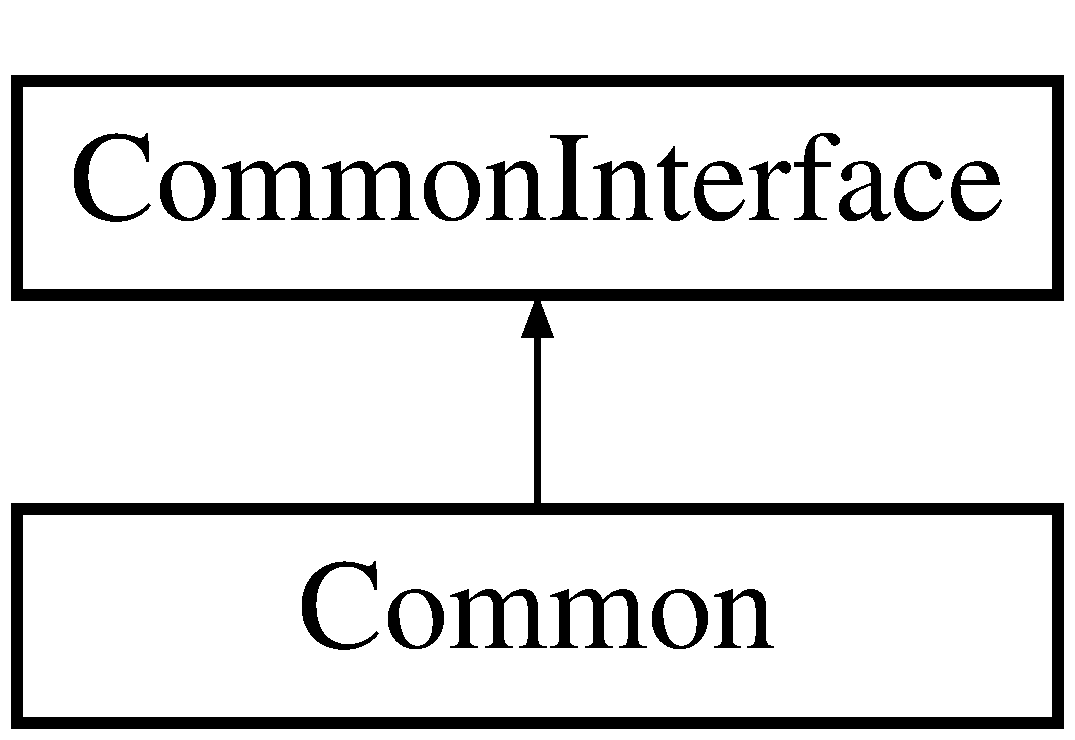
\includegraphics[height=2.000000cm]{class_common}
\end{center}
\end{figure}
\subsection*{Public Member Functions}
\begin{DoxyCompactItemize}
\item 
{\bf Common} (\$debug)
\item 
{\bf connect} (\$db)
\item 
{\bf execute\+Query} (\$sql, \$filename)
\end{DoxyCompactItemize}
\subsection*{Data Fields}
\begin{DoxyCompactItemize}
\item 
{\bf \$conn}
\item 
{\bf \$debug}
\item 
{\bf \$db} =\char`\"{}database.\+cse.\+tamu.\+edu\char`\"{}
\item 
{\bf \$dbname} =\char`\"{}jgwesterfield-\/Walker\+Data\char`\"{}
\item 
{\bf \$user} =\char`\"{}jgwesterfield\char`\"{}
\item 
{\bf \$pass} =\char`\"{}Whoop19!\char`\"{}
\end{DoxyCompactItemize}


\subsection{Detailed Description}
Created by Php\+Storm. User\+: Jonathan\+Westerfield Date\+: 2/8/18 Time\+: 4\+:20 PM 

Definition at line 9 of file Common\+Methods.\+php.



\subsection{Member Function Documentation}
\index{Common@{Common}!Common@{Common}}
\index{Common@{Common}!Common@{Common}}
\subsubsection[{Common(\$debug)}]{\setlength{\rightskip}{0pt plus 5cm}{\bf Common} (
\begin{DoxyParamCaption}
\item[{}]{\$debug}
\end{DoxyParamCaption}
)}\label{class_common_a4a9e6769ab6c946d0895e8d987df1c10}


Implements {\bf Common\+Interface} \doxyref{}{p.}{interface_common_interface_a4a9e6769ab6c946d0895e8d987df1c10}.



Definition at line 25 of file Common\+Methods.\+php.

\index{Common@{Common}!connect@{connect}}
\index{connect@{connect}!Common@{Common}}
\subsubsection[{connect(\$db)}]{\setlength{\rightskip}{0pt plus 5cm}connect (
\begin{DoxyParamCaption}
\item[{}]{\$db}
\end{DoxyParamCaption}
)}\label{class_common_a1b1bd9b3f45a5fbd2549355282cdc96f}


Implements {\bf Common\+Interface} \doxyref{}{p.}{interface_common_interface_a1b1bd9b3f45a5fbd2549355282cdc96f}.



Definition at line 34 of file Common\+Methods.\+php.

\index{Common@{Common}!execute\+Query@{execute\+Query}}
\index{execute\+Query@{execute\+Query}!Common@{Common}}
\subsubsection[{execute\+Query(\$sql, \$filename)}]{\setlength{\rightskip}{0pt plus 5cm}execute\+Query (
\begin{DoxyParamCaption}
\item[{}]{\$sql, }
\item[{}]{\$filename}
\end{DoxyParamCaption}
)}\label{class_common_a57a9dbd1203cf7b3ef3c5ce40d4047cc}


Implements {\bf Common\+Interface} \doxyref{}{p.}{interface_common_interface_a57a9dbd1203cf7b3ef3c5ce40d4047cc}.



Definition at line 49 of file Common\+Methods.\+php.



\subsection{Field Documentation}
\index{Common@{Common}!\$conn@{\$conn}}
\index{\$conn@{\$conn}!Common@{Common}}
\subsubsection[{\$conn}]{\setlength{\rightskip}{0pt plus 5cm}\$conn}\label{class_common_aa8a5a87b9c1a6a0819b88447cbe41877}


Definition at line 11 of file Common\+Methods.\+php.

\index{Common@{Common}!\$db@{\$db}}
\index{\$db@{\$db}!Common@{Common}}
\subsubsection[{\$db}]{\setlength{\rightskip}{0pt plus 5cm}\$db =\char`\"{}database.\+cse.\+tamu.\+edu\char`\"{}}\label{class_common_a1fa3127fc82f96b1436d871ef02be319}


Definition at line 20 of file Common\+Methods.\+php.

\index{Common@{Common}!\$dbname@{\$dbname}}
\index{\$dbname@{\$dbname}!Common@{Common}}
\subsubsection[{\$dbname}]{\setlength{\rightskip}{0pt plus 5cm}\$dbname =\char`\"{}jgwesterfield-\/Walker\+Data\char`\"{}}\label{class_common_ac5111a571fffa2499732833bb7f0d8c1}


Definition at line 21 of file Common\+Methods.\+php.

\index{Common@{Common}!\$debug@{\$debug}}
\index{\$debug@{\$debug}!Common@{Common}}
\subsubsection[{\$debug}]{\setlength{\rightskip}{0pt plus 5cm}\$debug}\label{class_common_a85ae3e64cd40e9564adceb010085e9dd}


Definition at line 12 of file Common\+Methods.\+php.

\index{Common@{Common}!\$pass@{\$pass}}
\index{\$pass@{\$pass}!Common@{Common}}
\subsubsection[{\$pass}]{\setlength{\rightskip}{0pt plus 5cm}\$pass =\char`\"{}Whoop19!\char`\"{}}\label{class_common_a12ec2780b52bd1c54d38c2f981c0349f}


Definition at line 23 of file Common\+Methods.\+php.

\index{Common@{Common}!\$user@{\$user}}
\index{\$user@{\$user}!Common@{Common}}
\subsubsection[{\$user}]{\setlength{\rightskip}{0pt plus 5cm}\$user =\char`\"{}jgwesterfield\char`\"{}}\label{class_common_a598ca4e71b15a1313ec95f0df1027ca5}


Definition at line 22 of file Common\+Methods.\+php.



The documentation for this class was generated from the following file\+:\begin{DoxyCompactItemize}
\item 
Users/\+Jonathan\+Westerfield/\+Documents/\+C\+S\+C\+E 315/\+Rec\+Walker\+Counter/{\bf Common\+Methods.\+php}\end{DoxyCompactItemize}

\section{Common\+Interface Interface Reference}
\label{interface_common_interface}\index{Common\+Interface@{Common\+Interface}}
Inheritance diagram for Common\+Interface\+:\begin{figure}[H]
\begin{center}
\leavevmode
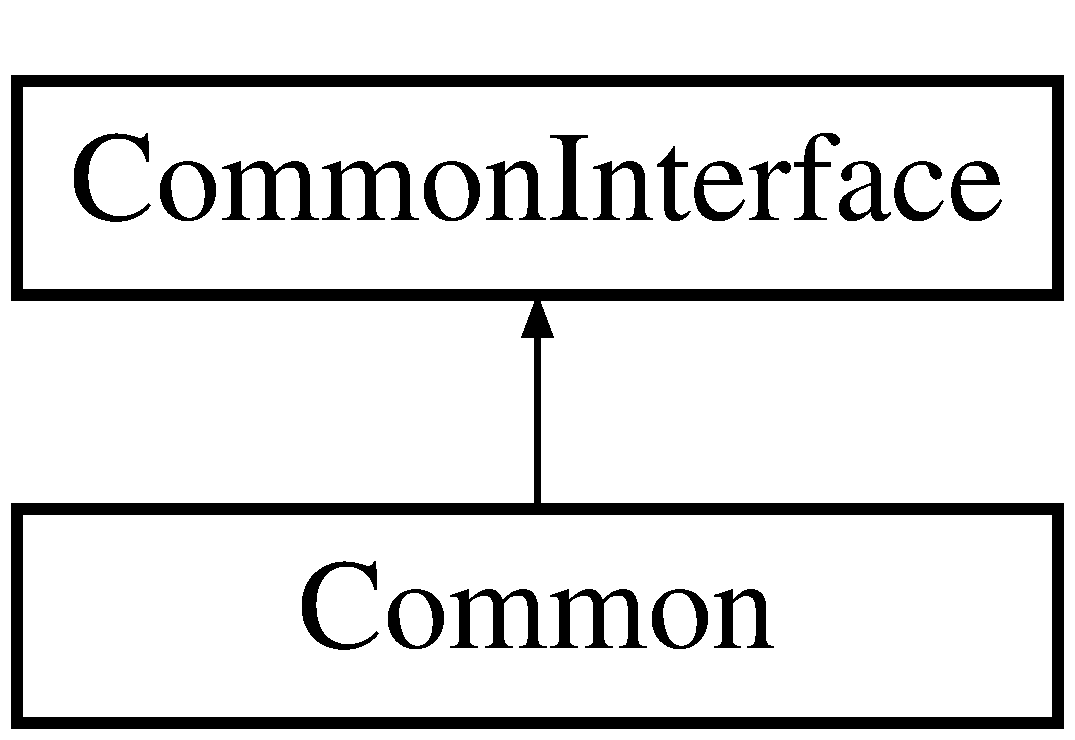
\includegraphics[height=2.000000cm]{interface_common_interface}
\end{center}
\end{figure}
\subsection*{Public Member Functions}
\begin{DoxyCompactItemize}
\item 
{\bfseries Common} (\$debug)\label{interface_common_interface_a4a9e6769ab6c946d0895e8d987df1c10}

\item 
{\bfseries connect} (\$db)\label{interface_common_interface_a1b1bd9b3f45a5fbd2549355282cdc96f}

\item 
{\bfseries execute\+Query} (\$sql, \$filename)\label{interface_common_interface_a57a9dbd1203cf7b3ef3c5ce40d4047cc}

\end{DoxyCompactItemize}


\subsection{Detailed Description}
Created by Php\+Storm. User\+: Jonathan\+Westerfield Date\+: 2/8/18 Time\+: 4\+:31 PM

This is an interface for \doxyref{Common}{p.}{class_common}. 

The documentation for this interface was generated from the following file\+:\begin{DoxyCompactItemize}
\item 
P\+H\+P\+:\+Mysql A\+P\+I/Common\+Interface.\+php\end{DoxyCompactItemize}

\section{D\+B\+A\+PI Class Reference}
\label{class_d_b_a_p_i}\index{D\+B\+A\+PI@{D\+B\+A\+PI}}
Inheritance diagram for D\+B\+A\+PI\+:\begin{figure}[H]
\begin{center}
\leavevmode
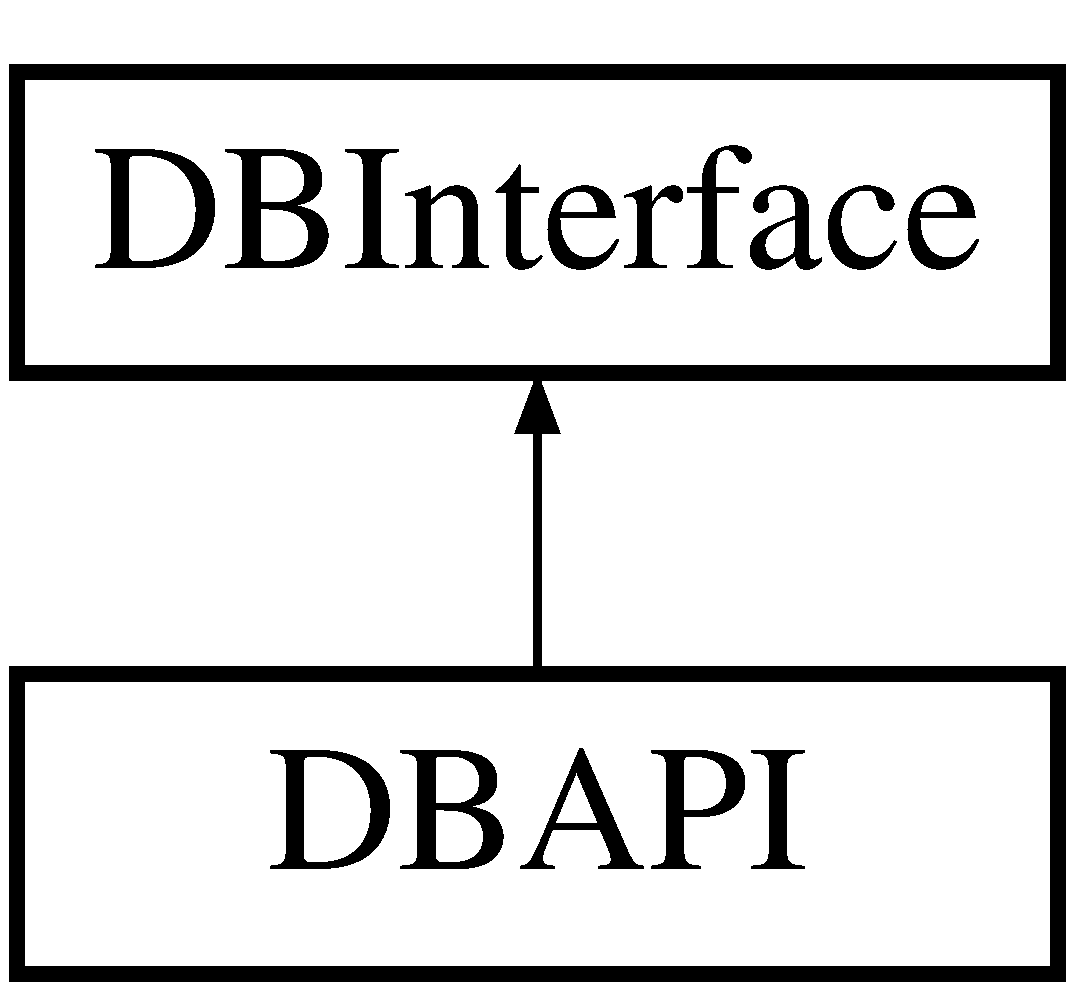
\includegraphics[height=2.000000cm]{class_d_b_a_p_i}
\end{center}
\end{figure}
\subsection*{Public Member Functions}
\begin{DoxyCompactItemize}
\item 
{\bf \+\_\+\+\_\+construct} (\$db)
\item 
{\bf \+\_\+\+\_\+destruct} ()
\item 
{\bf print\+Entire\+DB} ()
\item 
{\bf get\+Total\+Num\+Walkers} ()
\item 
{\bf get\+Num\+Walkers\+Today} ()
\item 
{\bf get\+Num\+Walkers\+This\+Week} ()
\item 
{\bf get\+Current\+Year\+Traffic} ()
\item 
{\bf get\+Traffic\+By\+Year} (\$year)
\item 
{\bf get\+Current\+Month\+Traffic} ()
\item 
{\bf get\+Traffic\+By\+Month} (\$year, \$month)
\item 
{\bf get\+Current\+Day\+Traffic} ()
\item 
{\bf get\+Traffic\+By\+Day} (\$year, \$month, \$day)
\item 
{\bf get\+Traffic\+Time\+Range} (\$year1, \$month1, \$day1, \$year2, \$month2, \$day2)
\end{DoxyCompactItemize}


\subsection{Detailed Description}
Created by Php\+Storm. User\+: Jonathan\+Westerfield Date\+: 2/8/18 Time\+: 4\+:35 PM

Includes the various functions that can be used in order to extract useful information from the database. Implements D\+B\+Interface.\+php 

\subsection{Constructor \& Destructor Documentation}
\index{D\+B\+A\+PI@{D\+B\+A\+PI}!\+\_\+\+\_\+construct@{\+\_\+\+\_\+construct}}
\index{\+\_\+\+\_\+construct@{\+\_\+\+\_\+construct}!D\+B\+A\+PI@{D\+B\+A\+PI}}
\subsubsection[{\+\_\+\+\_\+construct(\$db)}]{\setlength{\rightskip}{0pt plus 5cm}\+\_\+\+\_\+construct (
\begin{DoxyParamCaption}
\item[{}]{\$db}
\end{DoxyParamCaption}
)}\label{class_d_b_a_p_i_a800f8efee13692788b13ee57c5960092}
\doxyref{D\+B\+A\+PI}{p.}{class_d_b_a_p_i} constructor. 
\begin{DoxyParams}{Parameters}
{\em \$db} & Mostly sets up the dates in this object. Also sets the timezone to our timezone. \\
\hline
\end{DoxyParams}


Implements {\bf D\+B\+Interface} \doxyref{}{p.}{interface_d_b_interface_a800f8efee13692788b13ee57c5960092}.

\index{D\+B\+A\+PI@{D\+B\+A\+PI}!\+\_\+\+\_\+destruct@{\+\_\+\+\_\+destruct}}
\index{\+\_\+\+\_\+destruct@{\+\_\+\+\_\+destruct}!D\+B\+A\+PI@{D\+B\+A\+PI}}
\subsubsection[{\+\_\+\+\_\+destruct()}]{\setlength{\rightskip}{0pt plus 5cm}\+\_\+\+\_\+destruct (
\begin{DoxyParamCaption}
{}
\end{DoxyParamCaption}
)}\label{class_d_b_a_p_i_a421831a265621325e1fdd19aace0c758}
Class destructor 

Implements {\bf D\+B\+Interface} \doxyref{}{p.}{interface_d_b_interface}.



\subsection{Member Function Documentation}
\index{D\+B\+A\+PI@{D\+B\+A\+PI}!get\+Current\+Day\+Traffic@{get\+Current\+Day\+Traffic}}
\index{get\+Current\+Day\+Traffic@{get\+Current\+Day\+Traffic}!D\+B\+A\+PI@{D\+B\+A\+PI}}
\subsubsection[{get\+Current\+Day\+Traffic()}]{\setlength{\rightskip}{0pt plus 5cm}get\+Current\+Day\+Traffic (
\begin{DoxyParamCaption}
{}
\end{DoxyParamCaption}
)}\label{class_d_b_a_p_i_a50aa5202dd6a6314b4b0da6fd3026415}
\begin{DoxyReturn}{Returns}
array
\end{DoxyReturn}
Gets the number of people for every hour and returns a length 24 array output the times to see if I overshot how many times to iterate 

Implements {\bf D\+B\+Interface} \doxyref{}{p.}{interface_d_b_interface_a50aa5202dd6a6314b4b0da6fd3026415}.

\index{D\+B\+A\+PI@{D\+B\+A\+PI}!get\+Current\+Month\+Traffic@{get\+Current\+Month\+Traffic}}
\index{get\+Current\+Month\+Traffic@{get\+Current\+Month\+Traffic}!D\+B\+A\+PI@{D\+B\+A\+PI}}
\subsubsection[{get\+Current\+Month\+Traffic()}]{\setlength{\rightskip}{0pt plus 5cm}get\+Current\+Month\+Traffic (
\begin{DoxyParamCaption}
{}
\end{DoxyParamCaption}
)}\label{class_d_b_a_p_i_ae1b5c3c8112356b5c8ea9184286ec89a}
\begin{DoxyReturn}{Returns}
array
\end{DoxyReturn}
Gets the traffic numbers for each day during the current month. 

Implements {\bf D\+B\+Interface} \doxyref{}{p.}{interface_d_b_interface_ae1b5c3c8112356b5c8ea9184286ec89a}.

\index{D\+B\+A\+PI@{D\+B\+A\+PI}!get\+Current\+Year\+Traffic@{get\+Current\+Year\+Traffic}}
\index{get\+Current\+Year\+Traffic@{get\+Current\+Year\+Traffic}!D\+B\+A\+PI@{D\+B\+A\+PI}}
\subsubsection[{get\+Current\+Year\+Traffic()}]{\setlength{\rightskip}{0pt plus 5cm}get\+Current\+Year\+Traffic (
\begin{DoxyParamCaption}
{}
\end{DoxyParamCaption}
)}\label{class_d_b_a_p_i_ad487abf76c66536778a43009612b6843}
\begin{DoxyReturn}{Returns}
array
\end{DoxyReturn}
Returns an array of the traffic numbers for each month in a 12 element array 

Implements {\bf D\+B\+Interface} \doxyref{}{p.}{interface_d_b_interface_ad487abf76c66536778a43009612b6843}.

\index{D\+B\+A\+PI@{D\+B\+A\+PI}!get\+Num\+Walkers\+This\+Week@{get\+Num\+Walkers\+This\+Week}}
\index{get\+Num\+Walkers\+This\+Week@{get\+Num\+Walkers\+This\+Week}!D\+B\+A\+PI@{D\+B\+A\+PI}}
\subsubsection[{get\+Num\+Walkers\+This\+Week()}]{\setlength{\rightskip}{0pt plus 5cm}get\+Num\+Walkers\+This\+Week (
\begin{DoxyParamCaption}
{}
\end{DoxyParamCaption}
)}\label{class_d_b_a_p_i_ae7a2342889cfd984513ba17ddbd14bef}
\begin{DoxyReturn}{Returns}
int
\end{DoxyReturn}
Gets the number of walkers in the last week starting from today 

Implements {\bf D\+B\+Interface} \doxyref{}{p.}{interface_d_b_interface_ae7a2342889cfd984513ba17ddbd14bef}.

\index{D\+B\+A\+PI@{D\+B\+A\+PI}!get\+Num\+Walkers\+Today@{get\+Num\+Walkers\+Today}}
\index{get\+Num\+Walkers\+Today@{get\+Num\+Walkers\+Today}!D\+B\+A\+PI@{D\+B\+A\+PI}}
\subsubsection[{get\+Num\+Walkers\+Today()}]{\setlength{\rightskip}{0pt plus 5cm}get\+Num\+Walkers\+Today (
\begin{DoxyParamCaption}
{}
\end{DoxyParamCaption}
)}\label{class_d_b_a_p_i_adf40141a9763141c0eaeb9ce620181ad}
\begin{DoxyReturn}{Returns}
int
\end{DoxyReturn}
Gets the number of walkers from Today 

Implements {\bf D\+B\+Interface} \doxyref{}{p.}{interface_d_b_interface_adf40141a9763141c0eaeb9ce620181ad}.

\index{D\+B\+A\+PI@{D\+B\+A\+PI}!get\+Total\+Num\+Walkers@{get\+Total\+Num\+Walkers}}
\index{get\+Total\+Num\+Walkers@{get\+Total\+Num\+Walkers}!D\+B\+A\+PI@{D\+B\+A\+PI}}
\subsubsection[{get\+Total\+Num\+Walkers()}]{\setlength{\rightskip}{0pt plus 5cm}get\+Total\+Num\+Walkers (
\begin{DoxyParamCaption}
{}
\end{DoxyParamCaption}
)}\label{class_d_b_a_p_i_ab7a902c85d04b9973a30b73963cb3270}
\begin{DoxyReturn}{Returns}
int
\end{DoxyReturn}
Gets the total number of walkers in the table 

Implements {\bf D\+B\+Interface} \doxyref{}{p.}{interface_d_b_interface_ab7a902c85d04b9973a30b73963cb3270}.

\index{D\+B\+A\+PI@{D\+B\+A\+PI}!get\+Traffic\+By\+Day@{get\+Traffic\+By\+Day}}
\index{get\+Traffic\+By\+Day@{get\+Traffic\+By\+Day}!D\+B\+A\+PI@{D\+B\+A\+PI}}
\subsubsection[{get\+Traffic\+By\+Day(\$year, \$month, \$day)}]{\setlength{\rightskip}{0pt plus 5cm}get\+Traffic\+By\+Day (
\begin{DoxyParamCaption}
\item[{}]{\$year, }
\item[{}]{\$month, }
\item[{}]{\$day}
\end{DoxyParamCaption}
)}\label{class_d_b_a_p_i_a732a3a52aedfb5dd4b63f7292cb8ec3b}

\begin{DoxyParams}{Parameters}
{\em \$year} & \\
\hline
{\em \$month} & \\
\hline
{\em \$day} & \\
\hline
\end{DoxyParams}
\begin{DoxyReturn}{Returns}
array
\end{DoxyReturn}
Gets the traffic for each hour and returns it in a 24 element array.

Usage\+: $<$var = get\+Traffic\+By\+Day(2018, 2, 15);$>$ for Febraury 15, 2018 output the times to see if I overshot how many times to iterate 

Implements {\bf D\+B\+Interface} \doxyref{}{p.}{interface_d_b_interface_a732a3a52aedfb5dd4b63f7292cb8ec3b}.

\index{D\+B\+A\+PI@{D\+B\+A\+PI}!get\+Traffic\+By\+Month@{get\+Traffic\+By\+Month}}
\index{get\+Traffic\+By\+Month@{get\+Traffic\+By\+Month}!D\+B\+A\+PI@{D\+B\+A\+PI}}
\subsubsection[{get\+Traffic\+By\+Month(\$year, \$month)}]{\setlength{\rightskip}{0pt plus 5cm}get\+Traffic\+By\+Month (
\begin{DoxyParamCaption}
\item[{}]{\$year, }
\item[{}]{\$month}
\end{DoxyParamCaption}
)}\label{class_d_b_a_p_i_a0e954fca184f4b8ac04f51cb0c558def}

\begin{DoxyParams}{Parameters}
{\em \$year} & \\
\hline
{\em \$month} & \\
\hline
\end{DoxyParams}
\begin{DoxyReturn}{Returns}
array
\end{DoxyReturn}
Gets the traffic for each day during the specified month of the specified year

Usage\+: get\+Traffic\+By\+Month(2018, 2); // for February 2018 

Implements {\bf D\+B\+Interface} \doxyref{}{p.}{interface_d_b_interface_a0e954fca184f4b8ac04f51cb0c558def}.

\index{D\+B\+A\+PI@{D\+B\+A\+PI}!get\+Traffic\+By\+Year@{get\+Traffic\+By\+Year}}
\index{get\+Traffic\+By\+Year@{get\+Traffic\+By\+Year}!D\+B\+A\+PI@{D\+B\+A\+PI}}
\subsubsection[{get\+Traffic\+By\+Year(\$year)}]{\setlength{\rightskip}{0pt plus 5cm}get\+Traffic\+By\+Year (
\begin{DoxyParamCaption}
\item[{}]{\$year}
\end{DoxyParamCaption}
)}\label{class_d_b_a_p_i_a82c5e558141dca62c793baf0d1216bc0}

\begin{DoxyParams}{Parameters}
{\em \$year} & \\
\hline
\end{DoxyParams}
\begin{DoxyReturn}{Returns}
array
\end{DoxyReturn}
Gives the traffic for each month in an array for the specified year passed in 

Implements {\bf D\+B\+Interface} \doxyref{}{p.}{interface_d_b_interface_a82c5e558141dca62c793baf0d1216bc0}.

\index{D\+B\+A\+PI@{D\+B\+A\+PI}!get\+Traffic\+Time\+Range@{get\+Traffic\+Time\+Range}}
\index{get\+Traffic\+Time\+Range@{get\+Traffic\+Time\+Range}!D\+B\+A\+PI@{D\+B\+A\+PI}}
\subsubsection[{get\+Traffic\+Time\+Range(\$year1, \$month1, \$day1, \$year2, \$month2, \$day2)}]{\setlength{\rightskip}{0pt plus 5cm}get\+Traffic\+Time\+Range (
\begin{DoxyParamCaption}
\item[{}]{\$year1, }
\item[{}]{\$month1, }
\item[{}]{\$day1, }
\item[{}]{\$year2, }
\item[{}]{\$month2, }
\item[{}]{\$day2}
\end{DoxyParamCaption}
)}\label{class_d_b_a_p_i_a546615c71715e031c6218799e97937ab}

\begin{DoxyParams}{Parameters}
{\em \$year1} & \\
\hline
{\em \$month1} & \\
\hline
{\em \$day1} & \\
\hline
{\em \$year2} & \\
\hline
{\em \$month2} & \\
\hline
{\em \$day2} & \\
\hline
\end{DoxyParams}
\begin{DoxyReturn}{Returns}
int
\end{DoxyReturn}
Takes in a date range (start and end date) and counts the number of walkers in the given range 

Implements {\bf D\+B\+Interface} \doxyref{}{p.}{interface_d_b_interface_a546615c71715e031c6218799e97937ab}.

\index{D\+B\+A\+PI@{D\+B\+A\+PI}!print\+Entire\+DB@{print\+Entire\+DB}}
\index{print\+Entire\+DB@{print\+Entire\+DB}!D\+B\+A\+PI@{D\+B\+A\+PI}}
\subsubsection[{print\+Entire\+D\+B()}]{\setlength{\rightskip}{0pt plus 5cm}print\+Entire\+DB (
\begin{DoxyParamCaption}
{}
\end{DoxyParamCaption}
)}\label{class_d_b_a_p_i_a7e02b55449fecf4bed4ca717f38dafd5}
Prints out a table of the entire database 

Implements {\bf D\+B\+Interface} \doxyref{}{p.}{interface_d_b_interface}.



The documentation for this class was generated from the following file\+:\begin{DoxyCompactItemize}
\item 
P\+H\+P\+:\+Mysql A\+P\+I/D\+B\+A\+P\+I.\+php\end{DoxyCompactItemize}

\section{D\+B\+Interface Interface Reference}
\label{interface_d_b_interface}\index{D\+B\+Interface@{D\+B\+Interface}}
Inheritance diagram for D\+B\+Interface\+:\begin{figure}[H]
\begin{center}
\leavevmode
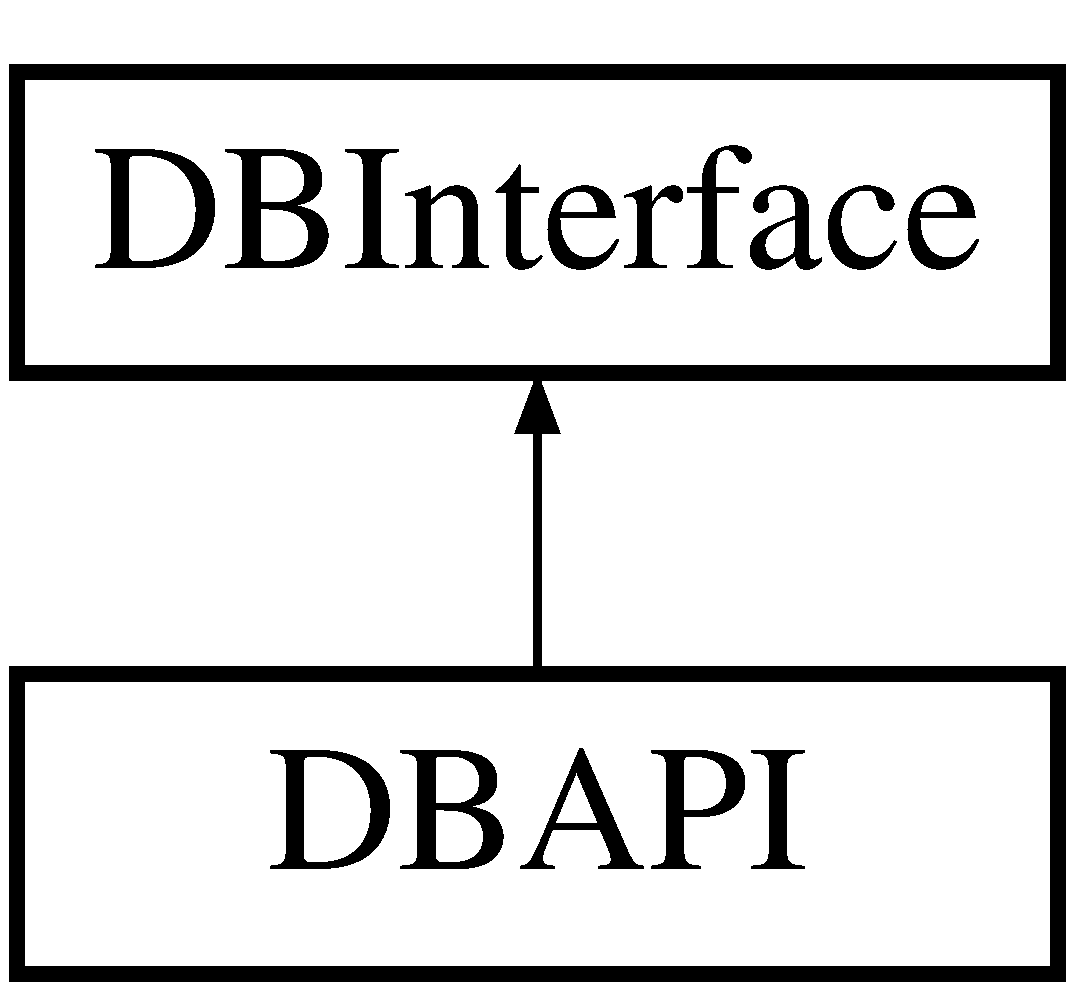
\includegraphics[height=2.000000cm]{interface_d_b_interface}
\end{center}
\end{figure}
\subsection*{Public Member Functions}
\begin{DoxyCompactItemize}
\item 
{\bf \+\_\+\+\_\+construct} (\$db)
\item 
{\bf \+\_\+\+\_\+destruct} ()
\item 
{\bf print\+Entire\+DB} ()
\item 
{\bf get\+Total\+Num\+Walkers} ()
\item 
{\bf get\+Num\+Walkers\+Today} ()
\item 
{\bf get\+Num\+Walkers\+This\+Week} ()
\item 
{\bf get\+Current\+Year\+Traffic} ()
\item 
{\bf get\+Traffic\+By\+Year} (\$year)
\item 
{\bf get\+Current\+Month\+Traffic} ()
\item 
{\bf get\+Traffic\+By\+Month} (\$year, \$month)
\item 
{\bf get\+Current\+Day\+Traffic} ()
\item 
{\bf get\+Traffic\+By\+Day} (\$year, \$month, \$day)
\item 
{\bf get\+Traffic\+Time\+Range} (\$year1, \$month1, \$day1, \$year2, \$month2, \$day2)
\end{DoxyCompactItemize}


\subsection{Detailed Description}
Created by Php\+Storm. User\+: Jonathan\+Westerfield Date\+: 2/8/18 Time\+: 4\+:36 PM 

Definition at line 11 of file D\+B\+Interface.\+php.



\subsection{Constructor \& Destructor Documentation}
\index{D\+B\+Interface@{D\+B\+Interface}!\+\_\+\+\_\+construct@{\+\_\+\+\_\+construct}}
\index{\+\_\+\+\_\+construct@{\+\_\+\+\_\+construct}!D\+B\+Interface@{D\+B\+Interface}}
\subsubsection[{\+\_\+\+\_\+construct(\$db)}]{\setlength{\rightskip}{0pt plus 5cm}\+\_\+\+\_\+construct (
\begin{DoxyParamCaption}
\item[{}]{\$db}
\end{DoxyParamCaption}
)}\label{interface_d_b_interface_a800f8efee13692788b13ee57c5960092}
\doxyref{D\+B\+A\+PI}{p.}{class_d_b_a_p_i} constructor. 
\begin{DoxyParams}{Parameters}
{\em \$db} & Mostly sets up the dates in this object. Also sets the timezone to our timezone. \\
\hline
\end{DoxyParams}


Implemented in {\bf D\+B\+A\+PI} \doxyref{}{p.}{class_d_b_a_p_i_a800f8efee13692788b13ee57c5960092}.

\index{D\+B\+Interface@{D\+B\+Interface}!\+\_\+\+\_\+destruct@{\+\_\+\+\_\+destruct}}
\index{\+\_\+\+\_\+destruct@{\+\_\+\+\_\+destruct}!D\+B\+Interface@{D\+B\+Interface}}
\subsubsection[{\+\_\+\+\_\+destruct()}]{\setlength{\rightskip}{0pt plus 5cm}\+\_\+\+\_\+destruct (
\begin{DoxyParamCaption}
{}
\end{DoxyParamCaption}
)}\label{interface_d_b_interface_a421831a265621325e1fdd19aace0c758}


Implemented in {\bf D\+B\+A\+PI} \doxyref{}{p.}{class_d_b_a_p_i_a421831a265621325e1fdd19aace0c758}.



\subsection{Member Function Documentation}
\index{D\+B\+Interface@{D\+B\+Interface}!get\+Current\+Day\+Traffic@{get\+Current\+Day\+Traffic}}
\index{get\+Current\+Day\+Traffic@{get\+Current\+Day\+Traffic}!D\+B\+Interface@{D\+B\+Interface}}
\subsubsection[{get\+Current\+Day\+Traffic()}]{\setlength{\rightskip}{0pt plus 5cm}get\+Current\+Day\+Traffic (
\begin{DoxyParamCaption}
{}
\end{DoxyParamCaption}
)}\label{interface_d_b_interface_a50aa5202dd6a6314b4b0da6fd3026415}
\begin{DoxyReturn}{Returns}
array
\end{DoxyReturn}
Returns a length 24 array containing total number of walkers for each hour for the current day 

Implemented in {\bf D\+B\+A\+PI} \doxyref{}{p.}{class_d_b_a_p_i_a50aa5202dd6a6314b4b0da6fd3026415}.

\index{D\+B\+Interface@{D\+B\+Interface}!get\+Current\+Month\+Traffic@{get\+Current\+Month\+Traffic}}
\index{get\+Current\+Month\+Traffic@{get\+Current\+Month\+Traffic}!D\+B\+Interface@{D\+B\+Interface}}
\subsubsection[{get\+Current\+Month\+Traffic()}]{\setlength{\rightskip}{0pt plus 5cm}get\+Current\+Month\+Traffic (
\begin{DoxyParamCaption}
{}
\end{DoxyParamCaption}
)}\label{interface_d_b_interface_ae1b5c3c8112356b5c8ea9184286ec89a}
\begin{DoxyReturn}{Returns}
array
\end{DoxyReturn}
Returns an array containing total number of walkers for each day for the current month 

Implemented in {\bf D\+B\+A\+PI} \doxyref{}{p.}{class_d_b_a_p_i_ae1b5c3c8112356b5c8ea9184286ec89a}.

\index{D\+B\+Interface@{D\+B\+Interface}!get\+Current\+Year\+Traffic@{get\+Current\+Year\+Traffic}}
\index{get\+Current\+Year\+Traffic@{get\+Current\+Year\+Traffic}!D\+B\+Interface@{D\+B\+Interface}}
\subsubsection[{get\+Current\+Year\+Traffic()}]{\setlength{\rightskip}{0pt plus 5cm}get\+Current\+Year\+Traffic (
\begin{DoxyParamCaption}
{}
\end{DoxyParamCaption}
)}\label{interface_d_b_interface_ad487abf76c66536778a43009612b6843}
\begin{DoxyReturn}{Returns}
array
\end{DoxyReturn}
Returns an array containing total number of walkers for each month for the current year 12 Element Array 

Implemented in {\bf D\+B\+A\+PI} \doxyref{}{p.}{class_d_b_a_p_i_ad487abf76c66536778a43009612b6843}.

\index{D\+B\+Interface@{D\+B\+Interface}!get\+Num\+Walkers\+This\+Week@{get\+Num\+Walkers\+This\+Week}}
\index{get\+Num\+Walkers\+This\+Week@{get\+Num\+Walkers\+This\+Week}!D\+B\+Interface@{D\+B\+Interface}}
\subsubsection[{get\+Num\+Walkers\+This\+Week()}]{\setlength{\rightskip}{0pt plus 5cm}get\+Num\+Walkers\+This\+Week (
\begin{DoxyParamCaption}
{}
\end{DoxyParamCaption}
)}\label{interface_d_b_interface_ae7a2342889cfd984513ba17ddbd14bef}
\begin{DoxyReturn}{Returns}
int
\end{DoxyReturn}
Returns the number of walkers from the start to the end of the week 

Implemented in {\bf D\+B\+A\+PI} \doxyref{}{p.}{class_d_b_a_p_i_ae7a2342889cfd984513ba17ddbd14bef}.

\index{D\+B\+Interface@{D\+B\+Interface}!get\+Num\+Walkers\+Today@{get\+Num\+Walkers\+Today}}
\index{get\+Num\+Walkers\+Today@{get\+Num\+Walkers\+Today}!D\+B\+Interface@{D\+B\+Interface}}
\subsubsection[{get\+Num\+Walkers\+Today()}]{\setlength{\rightskip}{0pt plus 5cm}get\+Num\+Walkers\+Today (
\begin{DoxyParamCaption}
{}
\end{DoxyParamCaption}
)}\label{interface_d_b_interface_adf40141a9763141c0eaeb9ce620181ad}
\begin{DoxyReturn}{Returns}
int
\end{DoxyReturn}
Returns the number of walkers that walked through from the start to the end of the day 

Implemented in {\bf D\+B\+A\+PI} \doxyref{}{p.}{class_d_b_a_p_i_adf40141a9763141c0eaeb9ce620181ad}.

\index{D\+B\+Interface@{D\+B\+Interface}!get\+Total\+Num\+Walkers@{get\+Total\+Num\+Walkers}}
\index{get\+Total\+Num\+Walkers@{get\+Total\+Num\+Walkers}!D\+B\+Interface@{D\+B\+Interface}}
\subsubsection[{get\+Total\+Num\+Walkers()}]{\setlength{\rightskip}{0pt plus 5cm}get\+Total\+Num\+Walkers (
\begin{DoxyParamCaption}
{}
\end{DoxyParamCaption}
)}\label{interface_d_b_interface_ab7a902c85d04b9973a30b73963cb3270}
\begin{DoxyReturn}{Returns}
int
\end{DoxyReturn}
Returns the total number of walkers in the table 

Implemented in {\bf D\+B\+A\+PI} \doxyref{}{p.}{class_d_b_a_p_i_ab7a902c85d04b9973a30b73963cb3270}.

\index{D\+B\+Interface@{D\+B\+Interface}!get\+Traffic\+By\+Day@{get\+Traffic\+By\+Day}}
\index{get\+Traffic\+By\+Day@{get\+Traffic\+By\+Day}!D\+B\+Interface@{D\+B\+Interface}}
\subsubsection[{get\+Traffic\+By\+Day(\$year, \$month, \$day)}]{\setlength{\rightskip}{0pt plus 5cm}get\+Traffic\+By\+Day (
\begin{DoxyParamCaption}
\item[{}]{\$year, }
\item[{}]{\$month, }
\item[{}]{\$day}
\end{DoxyParamCaption}
)}\label{interface_d_b_interface_a732a3a52aedfb5dd4b63f7292cb8ec3b}

\begin{DoxyParams}{Parameters}
{\em \$year} & \\
\hline
{\em \$month} & \\
\hline
{\em \$day} & \\
\hline
\end{DoxyParams}
\begin{DoxyReturn}{Returns}
array
\end{DoxyReturn}
Returns an array (24) containing total number of walkers for each hour

Usage\+: $<$var = get\+Traffic\+By\+Day(2018, 2, 15);$>$ for Febraury 15, 2018 

Implemented in {\bf D\+B\+A\+PI} \doxyref{}{p.}{class_d_b_a_p_i_a732a3a52aedfb5dd4b63f7292cb8ec3b}.

\index{D\+B\+Interface@{D\+B\+Interface}!get\+Traffic\+By\+Month@{get\+Traffic\+By\+Month}}
\index{get\+Traffic\+By\+Month@{get\+Traffic\+By\+Month}!D\+B\+Interface@{D\+B\+Interface}}
\subsubsection[{get\+Traffic\+By\+Month(\$year, \$month)}]{\setlength{\rightskip}{0pt plus 5cm}get\+Traffic\+By\+Month (
\begin{DoxyParamCaption}
\item[{}]{\$year, }
\item[{}]{\$month}
\end{DoxyParamCaption}
)}\label{interface_d_b_interface_a0e954fca184f4b8ac04f51cb0c558def}

\begin{DoxyParams}{Parameters}
{\em \$year} & \\
\hline
{\em \$month} & \\
\hline
\end{DoxyParams}
\begin{DoxyReturn}{Returns}
array
\end{DoxyReturn}
Gets the traffic for each day during the specified month of the specified year

Usage\+: get\+Traffic\+By\+Month(2018, 2); // for February 2018 

Implemented in {\bf D\+B\+A\+PI} \doxyref{}{p.}{class_d_b_a_p_i_a0e954fca184f4b8ac04f51cb0c558def}.

\index{D\+B\+Interface@{D\+B\+Interface}!get\+Traffic\+By\+Year@{get\+Traffic\+By\+Year}}
\index{get\+Traffic\+By\+Year@{get\+Traffic\+By\+Year}!D\+B\+Interface@{D\+B\+Interface}}
\subsubsection[{get\+Traffic\+By\+Year(\$year)}]{\setlength{\rightskip}{0pt plus 5cm}get\+Traffic\+By\+Year (
\begin{DoxyParamCaption}
\item[{}]{\$year}
\end{DoxyParamCaption}
)}\label{interface_d_b_interface_a82c5e558141dca62c793baf0d1216bc0}

\begin{DoxyParams}{Parameters}
{\em \$year} & \\
\hline
\end{DoxyParams}
\begin{DoxyReturn}{Returns}
array
\end{DoxyReturn}
Gives the traffic for each month in an array for the specified year passed in 

Implemented in {\bf D\+B\+A\+PI} \doxyref{}{p.}{class_d_b_a_p_i_a82c5e558141dca62c793baf0d1216bc0}.

\index{D\+B\+Interface@{D\+B\+Interface}!get\+Traffic\+Time\+Range@{get\+Traffic\+Time\+Range}}
\index{get\+Traffic\+Time\+Range@{get\+Traffic\+Time\+Range}!D\+B\+Interface@{D\+B\+Interface}}
\subsubsection[{get\+Traffic\+Time\+Range(\$year1, \$month1, \$day1, \$year2, \$month2, \$day2)}]{\setlength{\rightskip}{0pt plus 5cm}get\+Traffic\+Time\+Range (
\begin{DoxyParamCaption}
\item[{}]{\$year1, }
\item[{}]{\$month1, }
\item[{}]{\$day1, }
\item[{}]{\$year2, }
\item[{}]{\$month2, }
\item[{}]{\$day2}
\end{DoxyParamCaption}
)}\label{interface_d_b_interface_a546615c71715e031c6218799e97937ab}

\begin{DoxyParams}{Parameters}
{\em \$year1} & \\
\hline
{\em \$month1} & \\
\hline
{\em \$day1} & \\
\hline
{\em \$year2} & \\
\hline
{\em \$month2} & \\
\hline
{\em \$day2} & \\
\hline
\end{DoxyParams}
\begin{DoxyReturn}{Returns}
int
\end{DoxyReturn}
Takes in a date range (start and end date) and counts the number of walkers in the given range 

Implemented in {\bf D\+B\+A\+PI} \doxyref{}{p.}{class_d_b_a_p_i_a546615c71715e031c6218799e97937ab}.

\index{D\+B\+Interface@{D\+B\+Interface}!print\+Entire\+DB@{print\+Entire\+DB}}
\index{print\+Entire\+DB@{print\+Entire\+DB}!D\+B\+Interface@{D\+B\+Interface}}
\subsubsection[{print\+Entire\+D\+B()}]{\setlength{\rightskip}{0pt plus 5cm}print\+Entire\+DB (
\begin{DoxyParamCaption}
{}
\end{DoxyParamCaption}
)}\label{interface_d_b_interface_a7e02b55449fecf4bed4ca717f38dafd5}


Implemented in {\bf D\+B\+A\+PI} \doxyref{}{p.}{class_d_b_a_p_i_a7e02b55449fecf4bed4ca717f38dafd5}.



The documentation for this interface was generated from the following file\+:\begin{DoxyCompactItemize}
\item 
{\bf D\+B\+Interface.\+php}\end{DoxyCompactItemize}

\chapter{File Documentation}
\section{Python2.7/\+Counter.py File Reference}
\label{_counter_8py}\index{Python2.\+7/\+Counter.\+py@{Python2.\+7/\+Counter.\+py}}
\subsection*{Namespaces}
\begin{DoxyCompactItemize}
\item 
 {\bf Counter}
\end{DoxyCompactItemize}
\subsection*{Functions}
\begin{DoxyCompactItemize}
\item 
def {\bf insert} (cnx, cursor, in\+Or\+Out)
\item 
def {\bf db\+Connect} ()
\item 
def {\bf signal\+\_\+handler} (sig, frame)
\end{DoxyCompactItemize}
\subsection*{Variables}
\begin{DoxyCompactItemize}
\item 
{\bf board} = Py\+Mata(\char`\"{}C\+O\+M3\char`\"{}, verbose=True)
\item 
{\bf data} = board.\+get\+\_\+sonar\+\_\+data()
\item 
{\bf distance1} = data[12][1]
\item 
{\bf distance2} = data[13][1]
\item 
int {\bf hit1} = 0
\item 
int {\bf hit2} = 0
\item 
int {\bf dist} = 0
\end{DoxyCompactItemize}

\hypertarget{_common_interface_8php}{}\section{P\+H\+P-\/\+My\+S\+QL Source/\+Common\+Interface.php File Reference}
\label{_common_interface_8php}\index{P\+H\+P-\/\+My\+S\+Q\+L Source/\+Common\+Interface.\+php@{P\+H\+P-\/\+My\+S\+Q\+L Source/\+Common\+Interface.\+php}}
\subsection*{Data Structures}
\begin{DoxyCompactItemize}
\item 
interface \hyperlink{interface_common_interface}{Common\+Interface}
\end{DoxyCompactItemize}

\section{Common\+Methods.\+php File Reference}
\label{_common_methods_8php}\index{Common\+Methods.\+php@{Common\+Methods.\+php}}
\subsection*{Data Structures}
\begin{DoxyCompactItemize}
\item 
class {\bf Common}
\end{DoxyCompactItemize}

\hypertarget{_d_b_a_p_i_8php}{}\section{P\+H\+P-\/\+My\+S\+QL Source/\+D\+B\+A\+PI.php File Reference}
\label{_d_b_a_p_i_8php}\index{P\+H\+P-\/\+My\+S\+Q\+L Source/\+D\+B\+A\+P\+I.\+php@{P\+H\+P-\/\+My\+S\+Q\+L Source/\+D\+B\+A\+P\+I.\+php}}
\subsection*{Data Structures}
\begin{DoxyCompactItemize}
\item 
class \hyperlink{class_d_b_a_p_i}{D\+B\+A\+PI}
\end{DoxyCompactItemize}

\hypertarget{_d_b_interface_8php}{}\section{P\+H\+P-\/\+My\+S\+QL Source/\+D\+B\+Interface.php File Reference}
\label{_d_b_interface_8php}\index{P\+H\+P-\/\+My\+S\+Q\+L Source/\+D\+B\+Interface.\+php@{P\+H\+P-\/\+My\+S\+Q\+L Source/\+D\+B\+Interface.\+php}}
\subsection*{Data Structures}
\begin{DoxyCompactItemize}
\item 
interface \hyperlink{interface_d_b_interface}{D\+B\+Interface}
\end{DoxyCompactItemize}

\section{Users/\+Jonathan\+Westerfield/\+Documents/\+C\+S\+CE 315/\+Rec\+Walker\+Counter/\+Python/\+P\+D\+B\+A\+PI.py File Reference}
\label{_p_d_b_a_p_i_8py}\index{Users/\+Jonathan\+Westerfield/\+Documents/\+C\+S\+C\+E 315/\+Rec\+Walker\+Counter/\+Python/\+P\+D\+B\+A\+P\+I.\+py@{Users/\+Jonathan\+Westerfield/\+Documents/\+C\+S\+C\+E 315/\+Rec\+Walker\+Counter/\+Python/\+P\+D\+B\+A\+P\+I.\+py}}
\subsection*{Data Structures}
\begin{DoxyCompactItemize}
\item 
class {\bf P\+D\+B\+A\+PI}
\end{DoxyCompactItemize}
\subsection*{Namespaces}
\begin{DoxyCompactItemize}
\item 
 {\bf P\+D\+B\+A\+PI}
\end{DoxyCompactItemize}

\section{graph.\+php File Reference}
\label{graph_8php}\index{graph.\+php@{graph.\+php}}
\subsection*{Functions}
\begin{DoxyCompactItemize}
\item 
{\bf print\+\_\+array} (\$values)
\item 
{\bf display\+\_\+graph} (\$labels, \$values, \$date\+\_\+format)
\end{DoxyCompactItemize}
\subsection*{Variables}
\begin{DoxyCompactItemize}
\item 
{\bf \$this\+Common} = new {\bf Common}(true)
\item 
{\bf \$db} = new {\bf D\+B\+A\+PI}(\$this\+Common)
\item 
if(!isset(\$\+\_\+\+G\+ET[\textquotesingle{}mode\textquotesingle{}])) elseif(strtolower(\$\+\_\+\+G\+ET[\textquotesingle{}mode\textquotesingle{}])== \textquotesingle{}day\textquotesingle{}$\vert$$\vert$strtolower(\$\+\_\+\+G\+ET[\textquotesingle{}mode\textquotesingle{}])== \textquotesingle{}month\textquotesingle{}$\vert$$\vert$strtolower(\$\+\_\+\+G\+ET[\textquotesingle{}mode\textquotesingle{}])== \textquotesingle{}year\textquotesingle{}) {\bf else}
\end{DoxyCompactItemize}


\subsection{Function Documentation}
\index{graph.\+php@{graph.\+php}!display\+\_\+graph@{display\+\_\+graph}}
\index{display\+\_\+graph@{display\+\_\+graph}!graph.\+php@{graph.\+php}}
\subsubsection[{display\+\_\+graph(\$labels, \$values, \$date\+\_\+format)}]{\setlength{\rightskip}{0pt plus 5cm}display\+\_\+graph (
\begin{DoxyParamCaption}
\item[{}]{\$labels, }
\item[{}]{\$values, }
\item[{}]{\$date\+\_\+format}
\end{DoxyParamCaption}
)}\label{graph_8php_af55d8d11c9641c2dd1b0b29a790b0fe8}


Definition at line 24 of file graph.\+php.

\index{graph.\+php@{graph.\+php}!print\+\_\+array@{print\+\_\+array}}
\index{print\+\_\+array@{print\+\_\+array}!graph.\+php@{graph.\+php}}
\subsubsection[{print\+\_\+array(\$values)}]{\setlength{\rightskip}{0pt plus 5cm}print\+\_\+array (
\begin{DoxyParamCaption}
\item[{}]{\$values}
\end{DoxyParamCaption}
)}\label{graph_8php_a7af48d7091d5a774294eae9ab84a5057}


Definition at line 9 of file graph.\+php.



\subsection{Variable Documentation}
\index{graph.\+php@{graph.\+php}!\$db@{\$db}}
\index{\$db@{\$db}!graph.\+php@{graph.\+php}}
\subsubsection[{\$db}]{\setlength{\rightskip}{0pt plus 5cm}\$db = new {\bf D\+B\+A\+PI}(\$this\+Common)}\label{graph_8php_a1fa3127fc82f96b1436d871ef02be319}


Definition at line 7 of file graph.\+php.

\index{graph.\+php@{graph.\+php}!\$this\+Common@{\$this\+Common}}
\index{\$this\+Common@{\$this\+Common}!graph.\+php@{graph.\+php}}
\subsubsection[{\$this\+Common}]{\setlength{\rightskip}{0pt plus 5cm}\$this\+Common = new {\bf Common}(true)}\label{graph_8php_a2dc37683cec5a169d791007363950944}


Definition at line 6 of file graph.\+php.

\index{graph.\+php@{graph.\+php}!else@{else}}
\index{else@{else}!graph.\+php@{graph.\+php}}
\subsubsection[{else}]{\setlength{\rightskip}{0pt plus 5cm}if (!isset(\$\+\_\+\+G\+ET[\textquotesingle{}mode\textquotesingle{}])) elseif (strtolower(\$\+\_\+\+G\+ET[\textquotesingle{}mode\textquotesingle{}])== \textquotesingle{}day\textquotesingle{}$\vert$$\vert$strtolower(\$\+\_\+\+G\+ET[\textquotesingle{}mode\textquotesingle{}])== \textquotesingle{}month\textquotesingle{}$\vert$$\vert$strtolower(\$\+\_\+\+G\+ET[\textquotesingle{}mode\textquotesingle{}])== \textquotesingle{}year\textquotesingle{}) else}\label{graph_8php_aa98e5745136db21835880938c0eba666}
{\bfseries Initial value\+:}
\begin{DoxyCode}
\{

    echo \textcolor{stringliteral}{'<script>console.log("Could not load form with mode \(\backslash\)\(\backslash\)"'} . $\_GET[\textcolor{stringliteral}{'mode'}] . \textcolor{stringliteral}{'\(\backslash\)\(\backslash\)".");</script>'}
\end{DoxyCode}


Definition at line 106 of file graph.\+php.


\section{index.\+php File Reference}
\label{index_8php}\index{index.\+php@{index.\+php}}
\subsection*{Variables}
\begin{DoxyCompactItemize}
\item 
{\bf \$this\+Common} = new {\bf Common}(true)
\item 
{\bf \$db} = new {\bf D\+B\+A\+PI}(\$this\+Common)
\end{DoxyCompactItemize}


\subsection{Variable Documentation}
\index{index.\+php@{index.\+php}!\$db@{\$db}}
\index{\$db@{\$db}!index.\+php@{index.\+php}}
\subsubsection[{\$db}]{\setlength{\rightskip}{0pt plus 5cm}\$db = new {\bf D\+B\+A\+PI}(\$this\+Common)}\label{index_8php_a1fa3127fc82f96b1436d871ef02be319}


Definition at line 6 of file index.\+php.

\index{index.\+php@{index.\+php}!\$this\+Common@{\$this\+Common}}
\index{\$this\+Common@{\$this\+Common}!index.\+php@{index.\+php}}
\subsubsection[{\$this\+Common}]{\setlength{\rightskip}{0pt plus 5cm}\$this\+Common = new {\bf Common}(true)}\label{index_8php_a2dc37683cec5a169d791007363950944}


Definition at line 5 of file index.\+php.


\section{stats.\+php File Reference}
\label{stats_8php}\index{stats.\+php@{stats.\+php}}
\subsection*{Functions}
\begin{DoxyCompactItemize}
\item 
{\bf display\+\_\+stats} (\$date\+\_\+format, \$sub\+\_\+division, \$data)
\end{DoxyCompactItemize}
\subsection*{Variables}
\begin{DoxyCompactItemize}
\item 
{\bf \$this\+Common} = new {\bf Common}(true)
\item 
{\bf \$db} = new {\bf D\+B\+A\+PI}(\$this\+Common)
\item 
if(!isset(\$\+\_\+\+G\+ET[\textquotesingle{}mode\textquotesingle{}])) elseif(strtolower(\$\+\_\+\+G\+ET[\textquotesingle{}mode\textquotesingle{}])== \textquotesingle{}day\textquotesingle{}$\vert$$\vert$strtolower(\$\+\_\+\+G\+ET[\textquotesingle{}mode\textquotesingle{}])== \textquotesingle{}month\textquotesingle{}$\vert$$\vert$strtolower(\$\+\_\+\+G\+ET[\textquotesingle{}mode\textquotesingle{}])== \textquotesingle{}year\textquotesingle{}) {\bf else}
\end{DoxyCompactItemize}


\subsection{Function Documentation}
\index{stats.\+php@{stats.\+php}!display\+\_\+stats@{display\+\_\+stats}}
\index{display\+\_\+stats@{display\+\_\+stats}!stats.\+php@{stats.\+php}}
\subsubsection[{display\+\_\+stats(\$date\+\_\+format, \$sub\+\_\+division, \$data)}]{\setlength{\rightskip}{0pt plus 5cm}display\+\_\+stats (
\begin{DoxyParamCaption}
\item[{}]{\$date\+\_\+format, }
\item[{}]{\$sub\+\_\+division, }
\item[{}]{\$data}
\end{DoxyParamCaption}
)}\label{stats_8php_aadb6c25cd1cea1971104d049c282b778}


Definition at line 8 of file stats.\+php.



\subsection{Variable Documentation}
\index{stats.\+php@{stats.\+php}!\$db@{\$db}}
\index{\$db@{\$db}!stats.\+php@{stats.\+php}}
\subsubsection[{\$db}]{\setlength{\rightskip}{0pt plus 5cm}\$db = new {\bf D\+B\+A\+PI}(\$this\+Common)}\label{stats_8php_a1fa3127fc82f96b1436d871ef02be319}


Definition at line 6 of file stats.\+php.

\index{stats.\+php@{stats.\+php}!\$this\+Common@{\$this\+Common}}
\index{\$this\+Common@{\$this\+Common}!stats.\+php@{stats.\+php}}
\subsubsection[{\$this\+Common}]{\setlength{\rightskip}{0pt plus 5cm}\$this\+Common = new {\bf Common}(true)}\label{stats_8php_a2dc37683cec5a169d791007363950944}


Definition at line 5 of file stats.\+php.

\index{stats.\+php@{stats.\+php}!else@{else}}
\index{else@{else}!stats.\+php@{stats.\+php}}
\subsubsection[{else}]{\setlength{\rightskip}{0pt plus 5cm}if (!isset(\$\+\_\+\+G\+ET[\textquotesingle{}mode\textquotesingle{}])) elseif (strtolower(\$\+\_\+\+G\+ET[\textquotesingle{}mode\textquotesingle{}])== \textquotesingle{}day\textquotesingle{}$\vert$$\vert$strtolower(\$\+\_\+\+G\+ET[\textquotesingle{}mode\textquotesingle{}])== \textquotesingle{}month\textquotesingle{}$\vert$$\vert$strtolower(\$\+\_\+\+G\+ET[\textquotesingle{}mode\textquotesingle{}])== \textquotesingle{}year\textquotesingle{}) else}\label{stats_8php_aa98e5745136db21835880938c0eba666}
{\bfseries Initial value\+:}
\begin{DoxyCode}
\{
    echo \textcolor{stringliteral}{'<script>console.log("Could not load form with mode \(\backslash\)\(\backslash\)"'} . $\_GET[\textcolor{stringliteral}{'mode'}] . \textcolor{stringliteral}{'\(\backslash\)\(\backslash\)".");</script>'}
\end{DoxyCode}


Definition at line 48 of file stats.\+php.


%--- End generated contents ---

% Index
\backmatter
\newpage
\phantomsection
\clearemptydoublepage
\addcontentsline{toc}{chapter}{Index}
\printindex

\end{document}
